%%%%%%%%%%%%%%%%%%%%%%%%%%%%%%%%%%%%%%%%%
% Tufte Essay
% LaTeX Template
% Version 2.0 (19/1/19)
%
% This template originates from:
% http://www.LaTeXTemplates.com
%
% Authors:
% The Tufte-LaTeX Developers (https://www.ctan.org/pkg/tufte-latex)
% Vel (vel@LaTeXTemplates.com)
%
% License:
% Apache License, version 2.0
%
%%%%%%%%%%%%%%%%%%%%%%%%%%%%%%%%%%%%%%%%%

%----------------------------------------------------------------------------------------
%	PACKAGES AND OTHER DOCUMENT CONFIGURATIONS
%----------------------------------------------------------------------------------------

\documentclass{tufte-handout} % Use A4 paper by default, remove 'a4paper' for US letter

\usepackage{graphicx} % Required for including images
\setkeys{Gin}{width=\linewidth, totalheight=\textheight, keepaspectratio} % Default images settings
\graphicspath{{Figures/}{./}} % Specifies where to look for included images (trailing slash required)

\usepackage{booktabs} % Required for better horizontal rules in tables

\usepackage{subfiles}

\usepackage{pgfplots}
\pgfplotsset{compat=1.18}

%----------------------------------------------------------------------------------------
%	TITLE SECTION
%----------------------------------------------------------------------------------------

\title{Algebraic and Transcendental functions}

\author{Professor: Francisco Vazquez-Tavares}

\date{Last compilation: \today} % Date, use \date{} for no date


%----------------------------------------------------------------------------------------
%	COMMANDS SECTION
%----------------------------------------------------------------------------------------


%----------------------------------------------------------------------------------------

\begin{document}

\maketitle % Print the title section

%----------------------------------------------------------------------------------------
%	ABSTRACT/SUMMARY
%----------------------------------------------------------------------------------------

\begin{abstract}
    \textbf{\large Name: }\hfill November 14, 2025
\end{abstract}

%----------------------------------------------------------------------------------------
%	ESSAY BODY
%----------------------------------------------------------------------------------------


\marginpar{
    {\bfseries\Large Algebra Toolkit}

    {\bfseries\large Algebra properties}
    \begin{gather*}
        a+b = b+a, \\
        \qty(a+b)+c = a+\qty(b+c), \\
        a\qty(b+c) = ab+ac, \\
        \frac{a}{b} + \frac{c}{d} = \frac{ad+bc}{bd}, \quad
        \frac{a}{b} \cdot \frac{c}{d} = \frac{ac}{bd}, \\
        \frac{-a}{b} = -\frac{a}{b} = \frac{a}{-b}, \\
        \frac{\frac{a}{b}}{\frac{c}{d}} = \frac{ad}{bc}
        \\
        \sqrt{ab} = \sqrt{a}\sqrt{b},\quad
        \sqrt{\frac{a}{b}} = \frac{\sqrt{a}}{\sqrt{b}},\quad
        \sqrt[n]{a} = a^{1/n}
        \\
        x=\frac{-b\pm\sqrt{b^2-4ac}}{2a},\\
        a^2-b^2 = \qty(a-b)\qty(a+b)
    \end{gather*}
    
    {\bfseries\large Laws of exponents}
    \begin{align*}
        a^r\cdot a^s = a^{r+s}, \quad & \qty(a^r)^s = a^{rs} \\
        \frac{a^r}{a^s} = a^{r-s}, \quad & \qty(ab)^r = a^r b^r \\
        \qty(\frac{a}{b})^r = \frac{a^r}{b^r},\quad & b\neq 0
    \end{align*}

    {\bfseries\large Laws of Logarithms}
    \begin{align*}
        \log_a\qty(AB) &= \log_a\qty(A) + \log_a\qty(B) \\
        \log_a\qty(\frac{A}{B}) &= \log_a\qty(A) - \log_a\qty(B) \\
        \log_a\qty(A^C) &= C\log_a\qty(A)
    \end{align*}

    {\bfseries\large Inverse functions property}
    \begin{gather*}
        \qty(f\circ f^{-1})(x) = x = \qty(f^{-1}\circ f)(x) \\
        \log_a(a^x) = x = a^{\log_a(x)}
    \end{gather*}
}

\section{Algebra skills}

Use the complete the squared method to find the standard form of the the following conic sections,
\begin{align*}
    (a)\quad & 4x^2 + 9y^2 -8x +18y = -12 \\
    (b)\quad & 5x^2+5y^2-60x-20y+40=0 \\
    (c)\quad & -16x^2+9y-128x+18y-391=0
\end{align*}

\section{Function analysis}

Find the inverse function of the following function and find their domain and range,
\begin{align*}
    (a)\quad  f(x) = \sqrt{5-2x}, \qquad
    (b)\quad  g(x) = \frac{1}{x-2} \qquad
    (c)\quad  h(x) = \left(\frac{1}{2}\right)^{-x} + 2
\end{align*}



\section{Modelling with math}

\paragraph{Compound interest.} A total of \$3000 is invested at an annual interest of 5.4\%.
\begin{enumerate}
    \item Write the model of this situation.
    \item Find the balance after 3 years if it is compounded:
        \begin{itemize}
            \item Annually
            \item Montthly
            \item Daily
        \end{itemize}
    \item If the interest is compounded semiannually, hoy long will it triple your money?
\end{enumerate}

\paragraph{pH.} In the chemistry world, pH is used to describe the acidity and basicity of a substance through the equation $pH = -\log H$, $H$ being the concentration of hydrogen ions in moles per liter.
Jeffrey knows that avocados have $pH$ of 6.5, and chocolate has a $pH$ of 5.4. 
Based on this information, which of these two has a lower concentration of hydrogen ions? 

\section{Conic sections}
\marginpar{
    {\bfseries\Large Conic Sections}

    {\large Standard form of a circle}
    \begin{gather*}
        (x-h)^2 + (y-k)^2 = r^2
    \end{gather*}

    {\large Standard form of a parabola}
    \begin{gather*}
        (x-h) = 4a(y-k)^2,~\mathrm{or}~(y-k) = 4a(x-h)^2
    \end{gather*}

    {\large Standard form of an ellipse}
    \begin{gather*}
        \frac{(x-h)^2}{a^2} + \frac{(y-k)^2}{b^2} =1
    \end{gather*}

    {\large Standard form of a hyperbola}
    \begin{gather*}
        \frac{(x-h)^2}{a^2} - \frac{(y-k)^2}{b^2} =1
    \end{gather*}

}
Graph the following coninc sections,

\begin{gather*}
    1.\quad  x=-8(y-5)^2-1
\end{gather*}

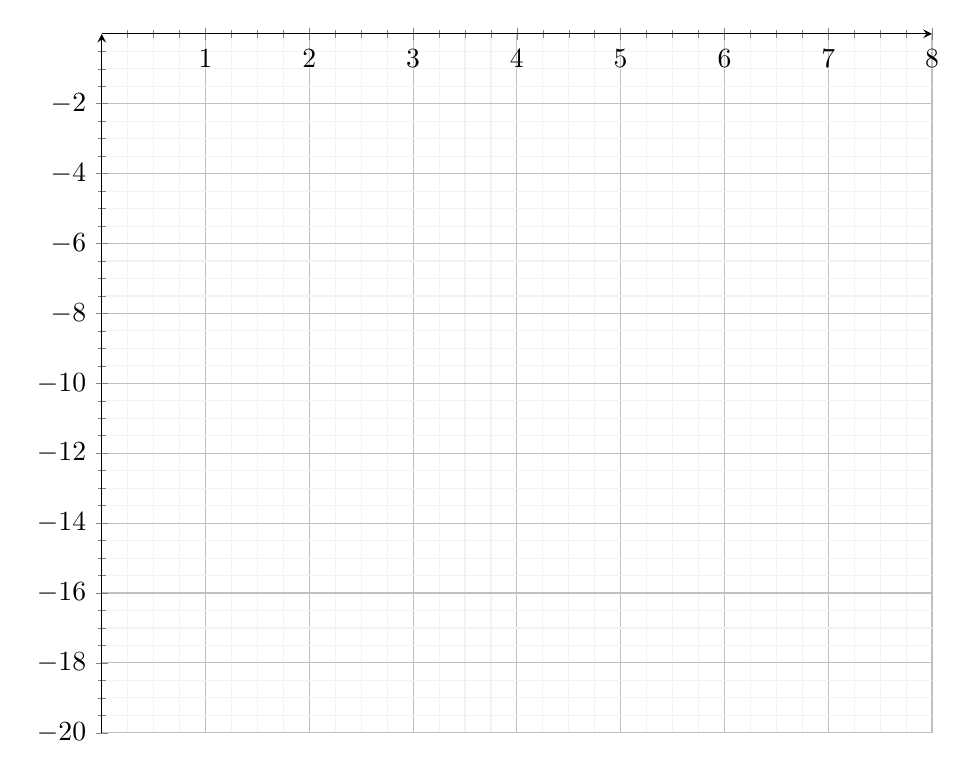
\begin{tikzpicture}
\begin{axis}[
    xmin=0, xmax=8,
    ymin=-20, ymax=0,
    grid=both,
    minor grid style={gray!10},  % Style for minor grid lines
    minor tick num=3,
    width=\textwidth,
    axis lines=center
]
% The axis environment automatically draws the grid based on the ticks
\end{axis}
\end{tikzpicture}

\begin{gather*}
    2.\quad  \frac{(x+5)^2}{4} - \frac{(y-4)^2}{25} = 1
\end{gather*}
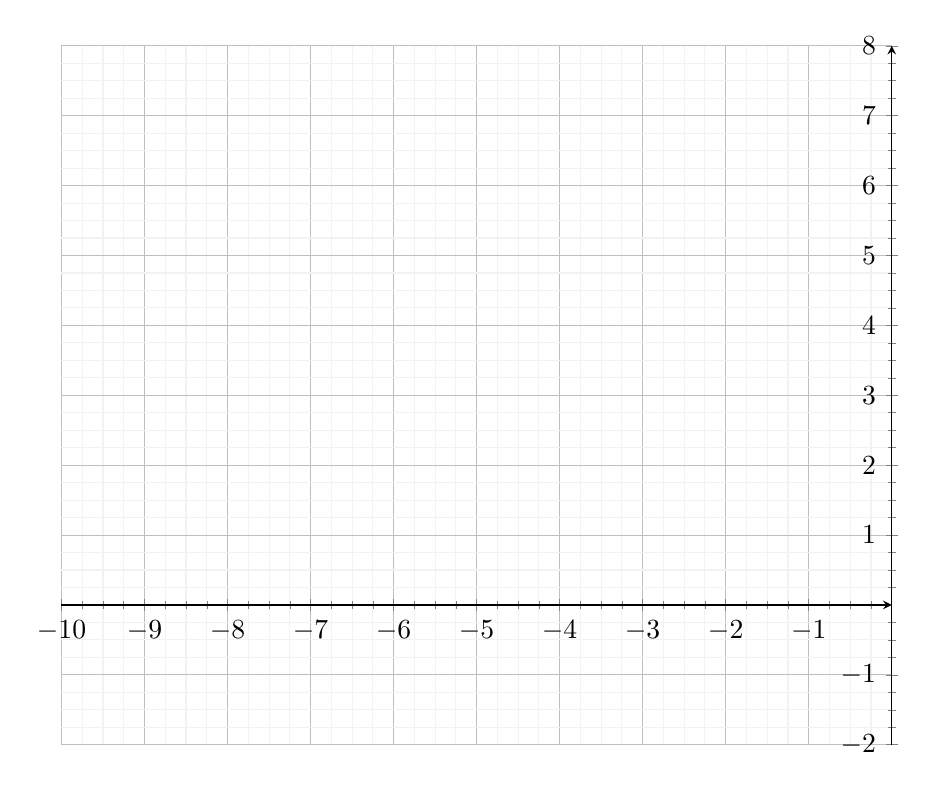
\begin{tikzpicture}
\begin{axis}[
    xmin=-10, xmax=0,
    ymin=-2, ymax=8,
    grid=both,
    minor grid style={gray!10},  % Style for minor grid lines
    minor tick num=3,
    width=\textwidth,
    axis lines=center
]
% The axis environment automatically draws the grid based on the ticks
\end{axis}
\end{tikzpicture}

\end{document}
